\usepackage[english]{babel}
\usepackage{indentfirst}
\usepackage[T1]{fontenc}
\usepackage[latin9]{inputenc}
\usepackage{nomencl}
\usepackage{amsmath}
\usepackage{graphicx}
\usepackage{listings}
\usepackage{color}
\usepackage{subfigure}
\usepackage{float}

%% ----------------------------------------------------------------------------
%% Defines the desired margins in the text
%% ----------------------------------------------------------------------------
\newlength{\margin}
\setlength{\margin}{2.5cm}

\setlength{\oddsidemargin}{\margin}
\setlength{\evensidemargin}{\margin}
\setlength{\textwidth}{\paperwidth}
\addtolength{\textwidth}{-\oddsidemargin}
\addtolength{\textwidth}{-\evensidemargin}

\setlength{\headsep}{\footskip}
\addtolength{\headsep}{-\headheight}
\addtolength{\headsep}{0.5cm}

\setlength{\topmargin}{\margin}
\setlength{\textheight}{\paperheight}
\addtolength{\textheight}{-\topmargin}
\addtolength{\textheight}{-\headheight}
\addtolength{\textheight}{-\headsep}
\addtolength{\textheight}{-\margin}
\addtolength{\textheight}{-\footskip}

\addtolength{\topmargin}{-1in}
\addtolength{\oddsidemargin}{-1in}
\addtolength{\evensidemargin}{-1in}

%% ----------------------------------------------------------------------------
%% Modifies some text metrics
%% ----------------------------------------------------------------------------
\renewcommand{\textfraction}{0.10}
\renewcommand{\topfraction}{0.90}
\renewcommand{\bottomfraction}{0.90}

%% ----------------------------------------------------------------------------
%% Defines commands for the titlepage and constructs the document name
%% ----------------------------------------------------------------------------
\newcommand{\foot}[1]{\newcommand{\@foot}{#1}}
\newcommand{\heading}[1]{\newcommand{\@heading}{#1}}
\newcommand{\city}[1]{\newcommand{\@city}{#1}}
\renewcommand{\month}[1]{\newcommand{\@month}{#1}}
\renewcommand{\year}[1]{\newcommand{\@year}{#1}}

%% ----------------------------------------------------------------------------
%% Defines spanish as the default language
%% ----------------------------------------------------------------------------
%%\RequirePackage[spanish]{babel}

%% ----------------------------------------------------------------------------
%% Modifies the header and foot styles of the pages
%% ----------------------------------------------------------------------------
\usepackage{fancyhdr}
\setlength{\headheight}{15.72pt}

\fancypagestyle{NanoStyle}{%
  \fancyhf{}%
  \renewcommand{\headrulewidth}{0.4pt}%
  \renewcommand{\footrulewidth}{0.4pt}%
  \fancyhead[LE]{\slshape\nouppercase{\leftmark}}%
  \fancyhead[RO]{\slshape\nouppercase{\rightmark}}%
  \fancyhead[RE,LO]{\@heading}%
  \fancyfoot[RE,LO]{\@foot}%
  \fancyfoot[LE,RO]{\thepage}}

\fancypagestyle{plain}{%
  \fancyhf{}%
  \renewcommand{\headrulewidth}{0pt}%
  \fancyfoot[LE,RO]{\thepage}}

\pagestyle{NanoStyle}

\renewcommand{\sectionmark}[1]{\markboth{\ifnum \thesection > 0 \thesection.\ \fi#1}%
                                        {\ifnum \thesection > 0 \thesection.\ \fi#1}}
\renewcommand{\subsectionmark}[1]{}

%% ----------------------------------------------------------------------------
%% Modifies the caption style
%% ----------------------------------------------------------------------------
\usepackage{caption}

\captionsetup{font=small,labelfont=bf}

%% ----------------------------------------------------------------------------
%% Redefines the \maketitle command
%% ----------------------------------------------------------------------------

\renewcommand{\maketitle}{%
  \begin{titlepage}%
    \renewcommand{\baselinestretch}{1.20} \normalsize%
    \begin{center}%
      {\LARGE \textbf{\@title}\\}%
      \vfill
      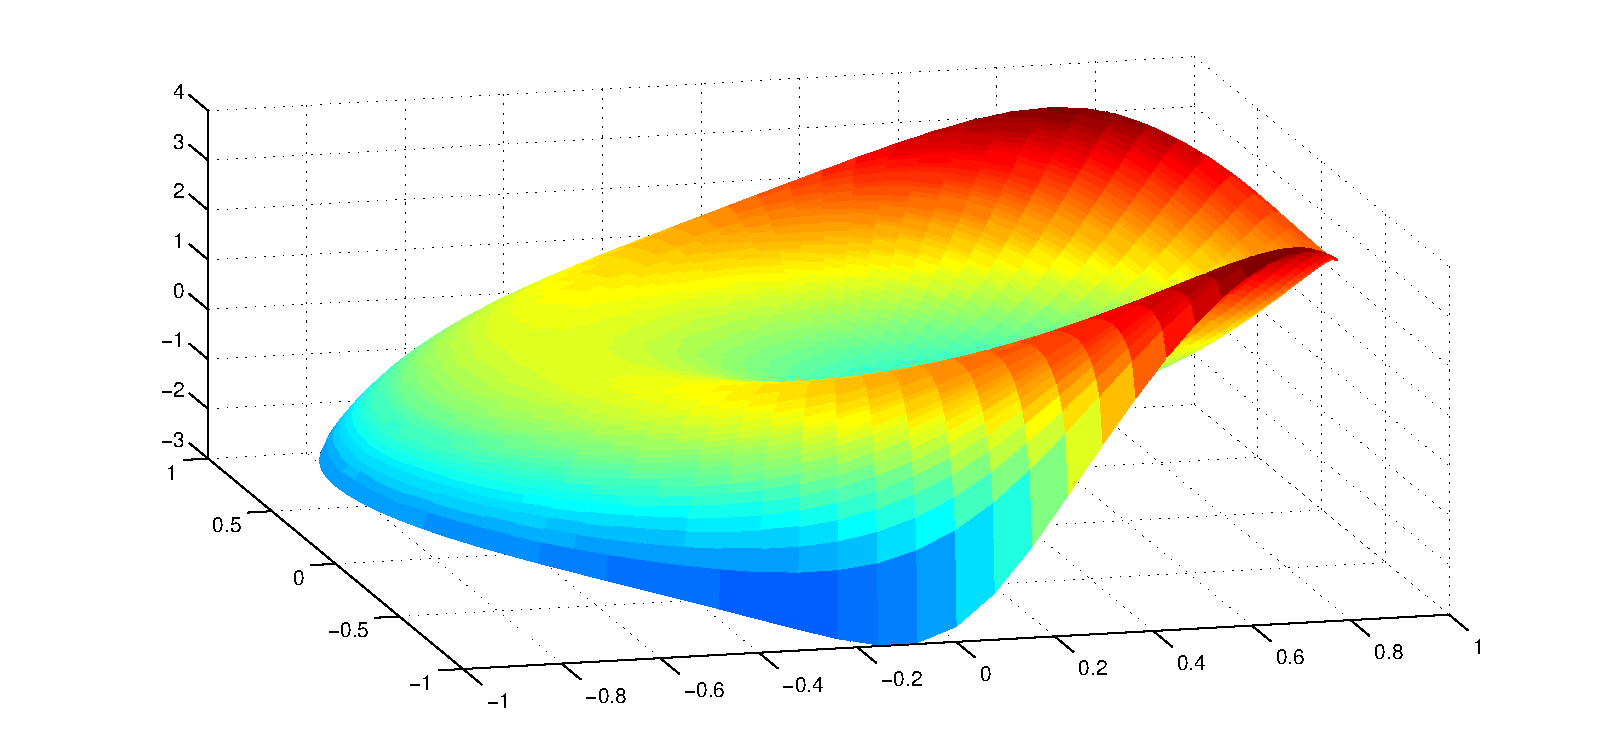
\includegraphics[width=0.65\textwidth]{portada}%
      \vfill
      {\large \bfseries \@author\\}%
      \vfill
      {\@city, \@month \, \@year \\}%
    \end{center}%
  \end{titlepage}%
  }

%% ----------------------------------------------------------------------------
%% Adds the References to the Table of Contents
%% ----------------------------------------------------------------------------
%\let\OLDtableofcontents=\tableofcontents
%\renewcommand{\tableofcontents}{%
%  \addcontentsline{toc}{section}{\contentsname}%
%  \OLDtableofcontents%
%  }

\newenvironment{resumen}{%
  \section*{Resumen}%
  \addcontentsline{toc}{section}{Resumen}%
  \sectionmark{Resumen}%
  }

\usepackage[nottoc]{tocbibind}
%%%%%%%%%%%%%%%%%%%%%%%%%%%%%%%%%%%%%%%%%%%%%%%%%%%%%%%%%%%%%%%%%%%%%%%%%%%%%%%
%%
%% FICHERO DE COMANDOS PARA ESCRIBIR MATEMATICAS EN TAS
%%
%% Creado por Oscar Lopez Abril 2008
%%
%% Recomendaciones generales
%%
%%   1. Abreviar con palabras de dos a tres letras
%%
%%   2. Nunca emplear numeros en la definicion del nombre de comando
%%      (no le gusta a LaTeX)
%%
%%   3. Las funciones con argumentos siempre se definen con los parentesis
%%      asociados a la forma de actuar.
%%
%%
%%
%%
%% General overview of alphabets
%%
%% b==bs==boldsymbol	computer modern
%% c==bc==boldsymbol	sans serif
%%%%%%%%%%%%%%%%%%%%%%%%%%%%%%%%%%%%%%%%%%%%%%%%%%%%%%%%%%%%%%%%%%%%%%%%%%%%%%%
%% Abreviacion de fuentes
%%%%%%%%%%%%%%%%%%%%%%%%%%%%%%%%%%%%%%%%%%%%%%%%%%%%%%%%%%%%%%%%%%%%%%%%%%%%%%%

\newcommand{\setArrayStretch}[1]{\renewcommand{\arraystretch}{#1}}
\newcommand{\unsetArrayStretch}{\renewcommand{\arraystretch}{1.0}}

%% NO DEFINIR bf ES PARA BOLDFACED
%   \newcommand{\boc}[1]{\ensuremath{\boldsymbol{\mathsf{#1}}}}
   \newcommand{\bbos}[1]{\ensuremath{\boldsymbol{#1}}}
   \newcommand{\bos}[1]{\ensuremath{\mathbf{#1}}}
   \newcommand{\boc}[1]{\ensuremath{\tilde{\mathsf{#1}}}}
%   \newcommand{\bos}[1]{\ensuremath{\vec{#1}}}

%%%%%%%%%%%%%%%%%%%%%%%%%%%%%%%%%%%%%%%%%%%%%%%%%%%%%%%%%%%%%%%%%%%%%%%%%%%%%%%
%% Abreviacion de operadores
%%%%%%%%%%%%%%%%%%%%%%%%%%%%%%%%%%%%%%%%%%%%%%%%%%%%%%%%%%%%%%%%%%%%%%%%%%%%%%%
   \newcommand{\abs}[1]{\lvert#1\rvert}
   \newcommand{\Asinh}[1]{\ensuremath{\mathrm{Asinh}#1}} %%  argument of hyperbolic sin
   \newcommand{\Acosh}[1]{\ensuremath{\mathrm{Acosh}#1}} %%  argument of hyperbolic cos
   \newcommand{\Atanh}[1]{\ensuremath{\mathrm{Atanh}#1}} %%  argument of hyperbolic tangent
   \newcommand{\atan}[1]{\ensuremath{\mathrm{arctan}#1}} %%  argument of circular tangent
%    \renewcommand{\det}[1]{\ensuremath{\mathrm{det}[#1]}} %% Determinant of a tensor 1 %% Desviador de un tensor 1
%    \renewcommand{\sin}[1]{\ensuremath{\mathrm{sen}#1}} %%  argument of circular tangent


%% Funciones
   \newcommand{\opname}[1]{\mathop{\mathrm{#1}}\nolimits}
   \newcommand{\sh}{\opname{Sh}}
   \newcommand{\ch}{\opname{Ch}}

   \newcommand{\D}{\ensuremath{\mathrm{d}}}
   \newcommand{\Ds}{\ensuremath{\mathrm{D}}}
   \newcommand{\img}{\ensuremath{\mathrm{i}}}


   \renewcommand\Re{\operatorname{Re}}
   \renewcommand\Im{\operatorname{Im}}
%   \newcommand{\ln}{\opname{ln}}

% Numeros adimensionales
   \newcommand{\Mach}{\ensuremath{\mathrm{M}}}
   \newcommand{\Rey}{\ensuremath{\mathrm{Re}}}

% Coeficientes y abreviaturas actuaciones
   \newcommand{\clmax}{\ensuremath{c_{l,\mathrm{max}}}}
%   \newcommand{\alphaclmax}{\ensuremath{\alpha_{cl,\mathrm{max}}}}
   \newcommand{\alphaclmax}{\ensuremath{\alpha_{s}}}
   \newcommand{\cdmin}{\ensuremath{c_{d,\mathrm{min}}}}
   \newcommand{\clcdmin}{\ensuremath{c_{l_{cd,\mathrm{min}}}}}
   \newcommand{\alphacdmin}{\ensuremath{\alpha_{cd,\mathrm{min}}}}
   \newcommand{\clopt}{\ensuremath{c_{l,\mathrm{opt}}}}
   \newcommand{\cdopt}{\ensuremath{c_{d,\mathrm{opt}}}}
   \newcommand{\alphaopt}{\ensuremath{\alpha_{\mathrm{opt}}}}
   \newcommand{\cdo}{\ensuremath{c_{d\mathrm{0}}}}
   \newcommand{\cLmax}{\ensuremath{c_{L,\mathrm{max}}}}
   \newcommand{\cDmin}{\ensuremath{c_{D,\mathrm{min}}}}
   \newcommand{\cDopt}{\ensuremath{c_{D,\mathrm{opt}}}}
   \newcommand{\cLopt}{\ensuremath{c_{L,\mathrm{opt}}}}
   \newcommand{\cDo}{\ensuremath{c_{D\mathrm{0}}}}

   \newcommand{\cpmin}{\ensuremath{c_{p,\mathrm{min}}}}
   \newcommand{\tmax}{\ensuremath{t_{\mathrm{max}}}}

   \newcommand{\cla}{\ensuremath{c_{l\alpha}}}
   \newcommand{\clo}{\ensuremath{c_{l0}}}

   \newcommand{\umin}{\ensuremath{u_{\infty,\mathrm{min}}}}
   \newcommand{\umax}{\ensuremath{u_{\infty,\mathrm{max}}}}

   \newcommand{\Emax}{\ensuremath{E_{\mathrm{max}}}}
   \newcommand{\clEmax}{\ensuremath{c_{l_{E,\mathrm{max}}}}}
   \newcommand{\cdEmax}{\ensuremath{c_{d_{E,\mathrm{max}}}}}
   \newcommand{\alphaEmax}{\ensuremath{\alpha_{E,\mathrm{max}}}}

   \newcommand{\nmax}{\ensuremath{n_{\mathrm{max}}}}

   \newcommand{\Rmin}{\ensuremath{R_{\mathrm{min}}}}


%%%%%%%%%%%%%%%%%%%%%%%%%%%%%%%%%%%%%%%%%%%%%%%%%%%%%%%%%%%%%%%%%%%%%%%%%%%%%%%
%% Abreviacion de simbolos vectores y tensores
%%%%%%%%%%%%%%%%%%%%%%%%%%%%%%%%%%%%%%%%%%%%%%%%%%%%%%%%%%%%%%%%%%%%%%%%%%%%%%%
%%
%%  Vectores, formas y tensores de sengundo orden
%%
%% b==bs==boldsymbol
   \newcommand{\bzero}{\bos{0}}
   \newcommand{\bA}{\bos{A}}
   \newcommand{\ba}{\bos{a}}
   \newcommand{\balpha}{\bbos{\alpha}}

   \newcommand{\bB}{\bos{B}}
   \newcommand{\bb}{\bos{b}}
   \newcommand{\bbeta}{\bbos{\beta}}

   \newcommand{\bC}{\bos{C}}
   \newcommand{\bc}{\bos{c}}
   \newcommand{\bchi}{\bbos{\chi}}

   \newcommand{\bD}{\bos{D}}
   \newcommand{\bd}{\bos{d}}
   \newcommand{\bdelta}{\bbos{\delta}}


   \newcommand{\bE}{\bos{E}}
   \newcommand{\be}{\bos{e}}
   \newcommand{\etab}{\bbos{\eta}}

   \newcommand{\bF}{\bos{F}}
   \newcommand{\bfi}{\bbos{\varphi}}
   \newcommand{\bfe}{\bos{f}}
%% NO DEFINIR bf ES PARA BOLDFACED

   \newcommand{\bG}{\bos{G}}
   \newcommand{\bg}{\bos{g}}
   \newcommand{\bGamma}{\bos{\Gamma}}
   \newcommand{\bgamma}{\bbos{\gamma}}

   \newcommand{\bH}{\bos{H}}
   \newcommand{\bh}{\bos{h}}

  \newcommand{\bi}{\bos{i}}
   \newcommand{\bId}{\bos{I}}
   \newcommand{\bI}{\bos{I}}

   \newcommand{\bJ}{\bos{J}}
   \newcommand{\bj}{\bos{j}}

   \newcommand{\bK}{\bos{K}}
   \newcommand{\bk}{\bos{k}}

   \newcommand{\bL}{\bos{L}}
   \newcommand{\bLambda}{\bos{\Lambda}}
   \newcommand{\blambda}{\bbos{\lambda}}
   \newcommand{\bl}{\bos{l}}

   \newcommand{\bM}{\bos{M}}
   \newcommand{\bma}{\bos{m}}
   \newcommand{\bmu}{\bbos{\mu}}

   \newcommand{\bN}{\bos{N}}
   \newcommand{\bn}{\bos{n}}
   \newcommand{\bnu}{\bbos{\nu}}

   \newcommand{\bO}{\bos{O}}
   \newcommand{\bo}{\bos{o}}
   \newcommand{\boeta}{\bos{\eta}}
   \newcommand{\bOmega}{\bos{\Omega}}
   \newcommand{\bomega}{\bbos{\omega}}

   \newcommand{\bP}{\bos{P}}
   \newcommand{\bp}{\bos{p}}
   \newcommand{\bphi}{\bbos{\phi}}
   \newcommand{\bPi}{\bos{\Pi}}

   \newcommand{\bQ}{\bos{Q}}
   \newcommand{\bq}{\bos{q}}

   \newcommand{\bR}{\bos{R}}
   \newcommand{\br}{\bos{r}}

   \newcommand{\bS}{\bos{S}}
%   \newcommand{\bs}{\bos{s}} % command clash with memoir
   \newcommand{\bsigma}{\bbos{\sigma}}
   \newcommand{\bSigma}{\bos{\Sigma}}

   \newcommand{\bT}{\bos{T}}
   \newcommand{\bTheta}{\bos{\Theta}}
   \newcommand{\bt}{\bos{t}}
   \newcommand{\btheta}{\bbos{\theta}}
   \newcommand{\btau}{\bbos{\tau}}

   \newcommand{\bU}{\bos{U}}
   \newcommand{\bu}{\bos{u}}
   \newcommand{\buno}{\bos{1}}

   \newcommand{\bV}{\bos{V}}
   \newcommand{\bv}{\bos{v}}

   \newcommand{\bW}{\bos{W}}
   \newcommand{\bw}{\bos{w}}

   \newcommand{\bX}{\bos{X}}
   \newcommand{\bXb}{\bar{\bX}}
   \newcommand{\bXi}{\bos{\Xi}}
   \newcommand{\bxi}{\bbos{\xi}}
   \newcommand{\bx}{\bos{x}}

   \newcommand{\bY}{\bos{Y}}
   \newcommand{\by}{\bos{y}}

   \newcommand{\bZ}{\bos{Z}}
   \newcommand{\bz}{\bos{z}}
   \newcommand{\bzeta}{\bbos{\zeta}}

%% c==bc==boldsymbol sans serif
   \newcommand{\cA}{\boc{A}}
   \newcommand{\ca}{\boc{a}}

   \newcommand{\cB}{\boc{B}}
   \newcommand{\cb}{\boc{b}}

   \newcommand{\cC}{\boc{C}}
   \newcommand{\cCb}{\bar{\cC}}
   \newcommand{\cc}{\boc{c}}

   \newcommand{\cD}{\boc{D}}
   \newcommand{\cd}{\boc{d}}

   \newcommand{\cE}{\boc{E}}
   \newcommand{\ce}{\boc{e}}

   \newcommand{\cF}{\boc{F}}
   \newcommand{\cf}{\boc{f}}

   \newcommand{\cG}{\boc{G}}
   \newcommand{\cg}{\boc{g}}

   \newcommand{\cH}{\boc{H}}

   \newcommand{\cI}{\boc{I}}
   \newcommand{\ci}{\boc{i}}

   \newcommand{\cJ}{\boc{J}}
   \newcommand{\cj}{\boc{j}}

   \newcommand{\cK}{\boc{K}}
   \newcommand{\ck}{\boc{k}}

   \newcommand{\cL}{\boc{L}}
   \newcommand{\cl}{\boc{l}}

   \newcommand{\cM}{\boc{M}}

   \newcommand{\cN}{\boc{N}}
   \newcommand{\cn}{\boc{n}}

   \newcommand{\cO}{\boc{O}}
   \newcommand{\co}{\boc{o}}

   \newcommand{\cP}{\boc{P}}
   \newcommand{\cp}{\boc{p}}

   \newcommand{\cQ}{\boc{Q}}
   \newcommand{\cq}{\boc{q}}

   \newcommand{\cR}{\boc{R}}


   \newcommand{\cS}{\boc{S}}
%   \newcommand{\cs}{\boc{s}} % command clash with memoir

   \newcommand{\cT}{\boc{T}}
   \newcommand{\ct}{\boc{t}}

   \newcommand{\cU}{\boc{U}}
   \newcommand{\cu}{\boc{u}}

   \newcommand{\cV}{\boc{V}}
   \newcommand{\cv}{\boc{v}}

   \newcommand{\cW}{\boc{W}}
   \newcommand{\cw}{\boc{w}}

   \newcommand{\cX}{\boc{X}}
   \newcommand{\cx}{\boc{x}}

   \newcommand{\cY}{\boc{Y}}
   \newcommand{\cy}{\boc{y}}

   \newcommand{\cZ}{\boc{Z}}
   \newcommand{\cz}{\boc{z}}

% Comandos particulares de la notacion de helicopteros
\newcommand{\FM}{FM}
\newcommand{\AI}{AI}
\newcommand{\Eb}{\mbox{E}_b}
\newcommand{\Ea}{\mbox{E}_a}


\newcommand{\xGB}{x_{\mbox{\scriptsize{GB}}}}

\newcommand{\xCG}{x_{\mbox{\scriptsize{CG}}}}
\newcommand{\yCG}{y_{\mbox{\scriptsize{CG}}}}
\newcommand{\zCG}{z_{\mbox{\scriptsize{CG}}}}

\newcommand{\XCG}{X_{\mbox{\scriptsize{CG}}}}
\newcommand{\YCG}{Y_{\mbox{\scriptsize{CG}}}}
\newcommand{\ZCG}{Z_{\mbox{\scriptsize{CG}}}}

\newcommand{\bVA}{\bV^{\mbox{\scriptsize{A}}}}
\newcommand{\bVP}{\bV^{\mbox{\scriptsize{P}}}}
\newcommand{\bVairA}{\bV^{\mbox{\scriptsize{air,A}}}}
\newcommand{\bVairP}{\bV^{\mbox{\scriptsize{air,P}}}}
\newcommand{\bVE}{\bV^{\mbox{\scriptsize{E}}}}
\newcommand{\bVGB}{\bV^{\mbox{\scriptsize{GB}}}}

\newcommand{\FiEbxAi}{F_{b,x_{A1}}^{i,\mbox{\scriptsize{E}}}}
\newcommand{\FiEbyAi}{F_{b,y_{A1}}^{i,\mbox{\scriptsize{E}}}}
\newcommand{\FiEbzAi}{F_{b,z_{A1}}^{i,\mbox{\scriptsize{E}}}}

\newcommand{\FaEbxAi}{F_{b,x_{A1}}^{a,\mbox{\scriptsize{E}}}}
\newcommand{\FaEbyAi}{F_{b,y_{A1}}^{a,\mbox{\scriptsize{E}}}}
\newcommand{\FaEbzAi}{F_{b,z_{A1}}^{a,\mbox{\scriptsize{E}}}}

\newcommand{\FabxAi}{F_{b,x_{A1}}^{a}}
\newcommand{\FabyAi}{F_{b,y_{A1}}^{a}}
\newcommand{\FabzAi}{F_{b,z_{A1}}^{a}}

\newcommand{\FibxAi}{F_{b,x_{A1}}^{i}}
\newcommand{\FibyAi}{F_{b,y_{A1}}^{i}}
\newcommand{\FibzAi}{F_{b,z_{A1}}^{i}}

\newcommand{\FtbxAi}{F_{b,x_{A1}}^{t}}
\newcommand{\FtbyAi}{F_{b,y_{A1}}^{t}}
\newcommand{\FtbzAi}{F_{b,z_{A1}}^{t}}

\newcommand{\bMaEb}{\bM_{b}^{a,\mbox{\scriptsize{E}}}}
\newcommand{\bMaEab}{\bM_{b}^{a,\mbox{\scriptsize{E}}_a}}
\newcommand{\bMaEastb}{\bM_{b}^{a,\mbox{\scriptsize{E*}}}}
\newcommand{\bMrEb}{\bM_{b}^{r,\mbox{\scriptsize{E}}}}
\newcommand{\bMtEb}{\bM_{b}^{t,\mbox{\scriptsize{E}}}}
\newcommand{\bMiEb}{\bM_{b}^{i,\mbox{\scriptsize{E}}}}
\newcommand{\bMtAb}{\bM_{b}^{t,\mbox{\scriptsize{A}}}}
\newcommand{\bMbFab}{\bM_{b}^{\bF^a}}
\newcommand{\bMbFib}{\bM_{b}^{\bF^i}}

\newcommand{\bmMtAb}{\overline{\bM}_{b}^{t,\mbox{\scriptsize{A}}}}
\newcommand{\bmMaEb}{\overline{\bM}_{b}^{a,\mbox{\scriptsize{E}}}}
\newcommand{\bmMaEastb}{\overline{\bM}_{b}^{a,\mbox{\scriptsize{E*}}}}
\newcommand{\bmMiEb}{\overline{\bM}_{b}^{i,\mbox{\scriptsize{E}}}}
\newcommand{\bmMbFab}{\overline{\bM}_{b}^{\bF^a}}
\newcommand{\bmMbFib}{\overline{\bM}_{b}^{\bF^i}}

\newcommand{\bmFtb}{\overline{\bF}_{b}^{t}}

\newcommand{\CaEaMxA}{C_{M_{x_{A}}}^{a,\mbox{\scriptsize{E*}}}}
\newcommand{\CaEaMyA}{C_{M_{y_{A}}}^{a,\mbox{\scriptsize{E*}}}}
\newcommand{\CaEaMzA}{C_{M_{z_{A}}}^{a,\mbox{\scriptsize{E*}}}}

\newcommand{\CaEMxA}{C_{M_{x_{A}}}^{a,\mbox{\scriptsize{E}}}}
\newcommand{\CaEMyA}{C_{M_{y_{A}}}^{a,\mbox{\scriptsize{E}}}}
\newcommand{\CaEMzA}{C_{M_{z_{A}}}^{a,\mbox{\scriptsize{E}}}}

\newcommand{\CbFaMxA}{C_{M_{x_{A}}}^{\bF^a}}
\newcommand{\CbFaMyA}{C_{M_{y_{A}}}^{\bF^a}}
\newcommand{\CbFaMzA}{C_{M_{z_{A}}}^{\bF^a}}

\newcommand{\mMaEbxAi}{\overline{M}_{b,x_{A1}}^{a,\mbox{\scriptsize{E}}}}
\newcommand{\mMaEbyAi}{\overline{M}_{b,y_{A1}}^{a,\mbox{\scriptsize{E}}}}
\newcommand{\mMaEbzAi}{\overline{M}_{b,z_{A1}}^{a,\mbox{\scriptsize{E}}}}

\newcommand{\mMbFabxAi}{\overline{M}_{b,x_{A1}}^{\bF^a}}
\newcommand{\mMbFabyAi}{\overline{M}_{b,y_{A1}}^{\bF^a}}
\newcommand{\mMbFabzAi}{\overline{M}_{b,z_{A1}}^{\bF^a}}

\newcommand{\mMaEbxA}{\overline{M}_{b,x_{A}}^{a,\mbox{\scriptsize{E}}}}
\newcommand{\mMaEbyA}{\overline{M}_{b,y_{A}}^{a,\mbox{\scriptsize{E}}}}
\newcommand{\mMaEbzA}{\overline{M}_{b,z_{A}}^{a,\mbox{\scriptsize{E}}}}
\newcommand{\mMaEbiA}{\overline{M}_{b,i_{A}}^{a,\mbox{\scriptsize{E}}}}

\newcommand{\mMaEbastxA}{\overline{M}_{b,x_{A}}^{a,\mbox{\scriptsize{E*}}}}
\newcommand{\mMaEbastyA}{\overline{M}_{b,y_{A}}^{a,\mbox{\scriptsize{E*}}}}
\newcommand{\mMaEbastzA}{\overline{M}_{b,z_{A}}^{a,\mbox{\scriptsize{E*}}}}
\newcommand{\mMaEbastiA}{\overline{M}_{b,i_{A}}^{a,\mbox{\scriptsize{E*}}}}

\newcommand{\mMbFabxA}{\overline{M}_{b,x_{A}}^{\bF^a}}
\newcommand{\mMbFabyA}{\overline{M}_{b,y_{A}}^{\bF^a}}
\newcommand{\mMbFabzA}{\overline{M}_{b,z_{A}}^{\bF^a}}
\newcommand{\mMbFabiA}{\overline{M}_{b,i_{A}}^{\bF^a}}

\newcommand{\mMiEbxA}{\overline{M}_{b,x_{A}}^{i,\mbox{\scriptsize{E}}}}
\newcommand{\mMiEbyA}{\overline{M}_{b,y_{A}}^{i,\mbox{\scriptsize{E}}}}
\newcommand{\mMiEbzA}{\overline{M}_{b,z_{A}}^{i,\mbox{\scriptsize{E}}}}

\newcommand{\mMbFibxA}{\overline{M}_{b,x_{A}}^{\bF^i}}
\newcommand{\mMbFibyA}{\overline{M}_{b,y_{A}}^{\bF^i}}
\newcommand{\mMbFibzA}{\overline{M}_{b,z_{A}}^{\bF^i}}

\newcommand{\mMtAbxA}{\overline{M}_{b,x_{A}}^{t,\mbox{\scriptsize{A}}}}
\newcommand{\mMtAbyA}{\overline{M}_{b,y_{A}}^{t,\mbox{\scriptsize{A}}}}
\newcommand{\mMtAbzA}{\overline{M}_{b,z_{A}}^{t,\mbox{\scriptsize{A}}}}

\newcommand{\MaEbij}{M_{b,i_{j}}^{a,\mbox{\scriptsize{E}}}}
\newcommand{\MaEbxAi}{M_{b,x_{A1}}^{a,\mbox{\scriptsize{E}}}}
\newcommand{\MaEbyAi}{M_{b,y_{A1}}^{a,\mbox{\scriptsize{E}}}}
\newcommand{\MaEbzAi}{M_{b,z_{A1}}^{a,\mbox{\scriptsize{E}}}}

\newcommand{\MaEbxA}{M_{b,x_{A}}^{a,\mbox{\scriptsize{E}}}}
\newcommand{\MaEbyA}{M_{b,y_{A}}^{a,\mbox{\scriptsize{E}}}}
\newcommand{\MaEbzA}{M_{b,z_{A}}^{a,\mbox{\scriptsize{E}}}}

\newcommand{\MaEastbiA}{M_{b,i_{A}}^{a,\mbox{\scriptsize{E*}}}}
\newcommand{\MaEastbxA}{M_{b,x_{A}}^{a,\mbox{\scriptsize{E*}}}}
\newcommand{\MaEastbyA}{M_{b,y_{A}}^{a,\mbox{\scriptsize{E*}}}}
\newcommand{\MaEastbzA}{M_{b,z_{A}}^{a,\mbox{\scriptsize{E*}}}}


\newcommand{\MaEabxA}{M_{b,x_{A}}^{a,\mbox{\scriptsize{E}}_a}}
\newcommand{\MaEabyA}{M_{b,y_{A}}^{a,\mbox{\scriptsize{E}}_a}}
\newcommand{\MaEabzA}{M_{b,z_{A}}^{a,\mbox{\scriptsize{E}}_a}}

\newcommand{\MtAbij}{M_{b,i_{j}}^{t,\mbox{\scriptsize{A}}}}
\newcommand{\MtAbxAi}{M_{b,x_{A1}}^{t,\mbox{\scriptsize{A}}}}
\newcommand{\MtAbyAi}{M_{b,y_{A1}}^{t,\mbox{\scriptsize{A}}}}
\newcommand{\MtAbzAi}{M_{b,z_{A1}}^{t,\mbox{\scriptsize{A}}}}

\newcommand{\MtAbxA}{M_{b,x_{A}}^{t,\mbox{\scriptsize{A}}}}
\newcommand{\MtAbyA}{M_{b,y_{A}}^{t,\mbox{\scriptsize{A}}}}
\newcommand{\MtAbzA}{M_{b,z_{A}}^{t,\mbox{\scriptsize{A}}}}

\newcommand{\MbFibxAi}{M_{b,x_{A1}}^{\bF^i}}
\newcommand{\MbFibyAi}{M_{b,y_{A1}}^{\bF^i}}
\newcommand{\MbFibzAi}{M_{b,z_{A1}}^{\bF^i}}

\newcommand{\MbFibij}{M_{b,i_{j}}^{\bF^i}}
\newcommand{\MbFibxA}{M_{b,x_{A}}^{\bF^i}}
\newcommand{\MbFibyA}{M_{b,y_{A}}^{\bF^i}}
\newcommand{\MbFibzA}{M_{b,z_{A}}^{\bF^i}}

\newcommand{\MbFabij}{M_{b,i_{j}}^{\bF^a}}
\newcommand{\MbFabxAi}{M_{b,x_{A1}}^{\bF^a}}
\newcommand{\MbFabyAi}{M_{b,y_{A1}}^{\bF^a}}
\newcommand{\MbFabzAi}{M_{b,z_{A1}}^{\bF^a}}

\newcommand{\MiEbij}{M_{b,i_{j}}^{i,\mbox{\scriptsize{E}}}}
\newcommand{\MiEbxAi}{M_{b,x_{A1}}^{i,\mbox{\scriptsize{E}}}}
\newcommand{\MiEbyAi}{M_{b,y_{A1}}^{i,\mbox{\scriptsize{E}}}}
\newcommand{\MiEbzAi}{M_{b,z_{A1}}^{i,\mbox{\scriptsize{E}}}}

\newcommand{\MiEbxA}{M_{b,x_{A}}^{i,\mbox{\scriptsize{E}}}}
\newcommand{\MiEbyA}{M_{b,y_{A}}^{i,\mbox{\scriptsize{E}}}}
\newcommand{\MiEbzA}{M_{b,z_{A}}^{i,\mbox{\scriptsize{E}}}}

\newcommand{\MtEbij}{M_{b,i_{j}}^{t,\mbox{\scriptsize{E}}}}
\newcommand{\MtEbxAi}{M_{b,x_{A1}}^{t,\mbox{\scriptsize{E}}}}
\newcommand{\MtEbyAi}{M_{b,y_{A1}}^{t,\mbox{\scriptsize{E}}}}
\newcommand{\MtEbzAi}{M_{b,z_{A1}}^{t,\mbox{\scriptsize{E}}}}

\newcommand{\MtEbxB}{M_{b,x_{B}}^{t,\mbox{\scriptsize{E}}}}
\newcommand{\MtEbyB}{M_{b,y_{B}}^{t,\mbox{\scriptsize{E}}}}
\newcommand{\MtEbzB}{M_{b,z_{B}}^{t,\mbox{\scriptsize{E}}}}

\newcommand{\MrEbij}{M_{b,i_{j}}^{r,\mbox{\scriptsize{E}}}}
\newcommand{\MrEbxB}{M_{b,x_{B}}^{r,\mbox{\scriptsize{E}}}}
\newcommand{\MrEbyB}{M_{b,y_{B}}^{r,\mbox{\scriptsize{E}}}}
\newcommand{\MrEbzB}{M_{b,z_{B}}^{r,\mbox{\scriptsize{E}}}}

\newcommand{\MrEbxAi}{M_{b,x_{A1}}^{r,\mbox{\scriptsize{E}}}}
\newcommand{\MrEbyAi}{M_{b,y_{A1}}^{r,\mbox{\scriptsize{E}}}}
\newcommand{\MrEbzAi}{M_{b,z_{A1}}^{r,\mbox{\scriptsize{E}}}}

\newcommand{\MrEbxAk}{M_{b,x_{A3}}^{r,\mbox{\scriptsize{E}}}}
\newcommand{\MrEbyAk}{M_{b,y_{A3}}^{r,\mbox{\scriptsize{E}}}}
\newcommand{\MrEbzAk}{M_{b,z_{A3}}^{r,\mbox{\scriptsize{E}}}}

\newcommand{\uAxA}{u_{x_{A}}^{\mbox{\scriptsize{A}}}}
\newcommand{\uAyA}{u_{y_{A}}^{\mbox{\scriptsize{A}}}}
\newcommand{\uAzA}{u_{z_{A}}^{\mbox{\scriptsize{A}}}}

\newcommand{\uAxi}{u_{x_{i}}^{\mbox{\scriptsize{A}}}}
\newcommand{\uAyi}{u_{y_{i}}^{\mbox{\scriptsize{A}}}}
\newcommand{\uAzi}{u_{z_{i}}^{\mbox{\scriptsize{A}}}}

\newcommand{\uAjA}{u_{j_{A}}^{\mbox{\scriptsize{A}}}}

\newcommand{\uAxP}{u_{x_{P}}^{\mbox{\scriptsize{A}}}}
\newcommand{\uAyP}{u_{y_{P}}^{\mbox{\scriptsize{A}}}}
\newcommand{\uAzP}{u_{z_{P}}^{\mbox{\scriptsize{A}}}}

\newcommand{\uAij}{u_{i_{j}}^{\mbox{\scriptsize{A}}}}

\newcommand{\uGBiA}{u_{i_{A}}^{\mbox{\scriptsize{GB}}}}
\newcommand{\uGBxA}{u_{x_{A}}^{\mbox{\scriptsize{GB}}}}
\newcommand{\uGByA}{u_{y_{A}}^{\mbox{\scriptsize{GB}}}}
\newcommand{\uGBzA}{u_{z_{A}}^{\mbox{\scriptsize{GB}}}}

\newcommand{\aGBiA}{a_{i_{A}}^{\mbox{\scriptsize{GB}}}}
\newcommand{\aGBxA}{a_{x_{A}}^{\mbox{\scriptsize{GB}}}}
\newcommand{\aGByA}{a_{y_{A}}^{\mbox{\scriptsize{GB}}}}
\newcommand{\aGBzA}{a_{z_{A}}^{\mbox{\scriptsize{GB}}}}



% Definiciones geometricas de vectores posicion
\newcommand{\bAEb}{\bos{AE}_b}
\newcommand{\bAP}{\bos{AP}}
\newcommand{\bAR}{\bos{AR}}
\newcommand{\bAE}{\bos{AE}}
\newcommand{\bEGB}{\bos{EGB}}
\newcommand{\bOA}{\bos{OA}}
\newcommand{\bOfA}{\bos{O}_f\bos{A}}
\newcommand{\bOE}{\bos{OE}}
\newcommand{\bOS}{\bos{OS}}
\newcommand{\bEP}{\bos{E}\bos{P}}
\newcommand{\bEaP}{\bos{E}_a\bos{P}}
\newcommand{\bEbP}{\bos{E}_b\bos{P}}
\newcommand{\bEbEa}{\bos{E}_b\bos{E}_a}

\newcommand{\brO}{\bos{r}^{\mbox{\scriptsize{O}}}}
\newcommand{\bOO}{\bos{O}\bos{O}}
\newcommand{\bOfO}{\bos{O}_f\bos{O}}
\newcommand{\bOfS}{\bos{O}_f\bos{S}}
\newcommand{\bOfAa}{\bos{O}_f\bos{A}_a}
\newcommand{\bOfEh}{\bos{O}_f\bos{E}_h}
\newcommand{\bOfEv}{\bos{O}_f\bos{E}_v}
\newcommand{\xRA}{x_{A}^{\mbox{\scriptsize{R}}}}
\newcommand{\yRA}{y_{A}^{\mbox{\scriptsize{R}}}}
\newcommand{\zRA}{z_{A}^{\mbox{\scriptsize{R}}}}


\usepackage{hyperref}
\hypersetup{
  colorlinks=true,
  linkcolor=black,
  filecolor=black,
  citecolor=black,
  pdftitle={Heroes},
  pdfsubject={},
  pdfauthor={\'{A}lvaro Cuerva, \'{O}scar L\'{o}pez, Mariano Rubio},
  pdfkeywords={},
  bookmarksopen=true
}
